% !TeX root = ./testing.tex
\documentclass[../../report.tex]{subfiles}

\begin{document}

\chapter{Testing summary}
The chess recognition pipeline has been extensively tested. 
Three main methods of testing were employed to ensure the quality of the system: 
\begin{enumerate}
    \item manual end-to-end testing by means of the web app demonstration;
    \item performing an empirical evaluation of the different components in the pipeline and the system as a whole; and
    \item running automated unit tests in all three repositories.
\end{enumerate}
For the first point, \cref{fig:chesscogapp_inference} shows the result of a chess position inference using the web app.
\begin{figure}
    \centering
    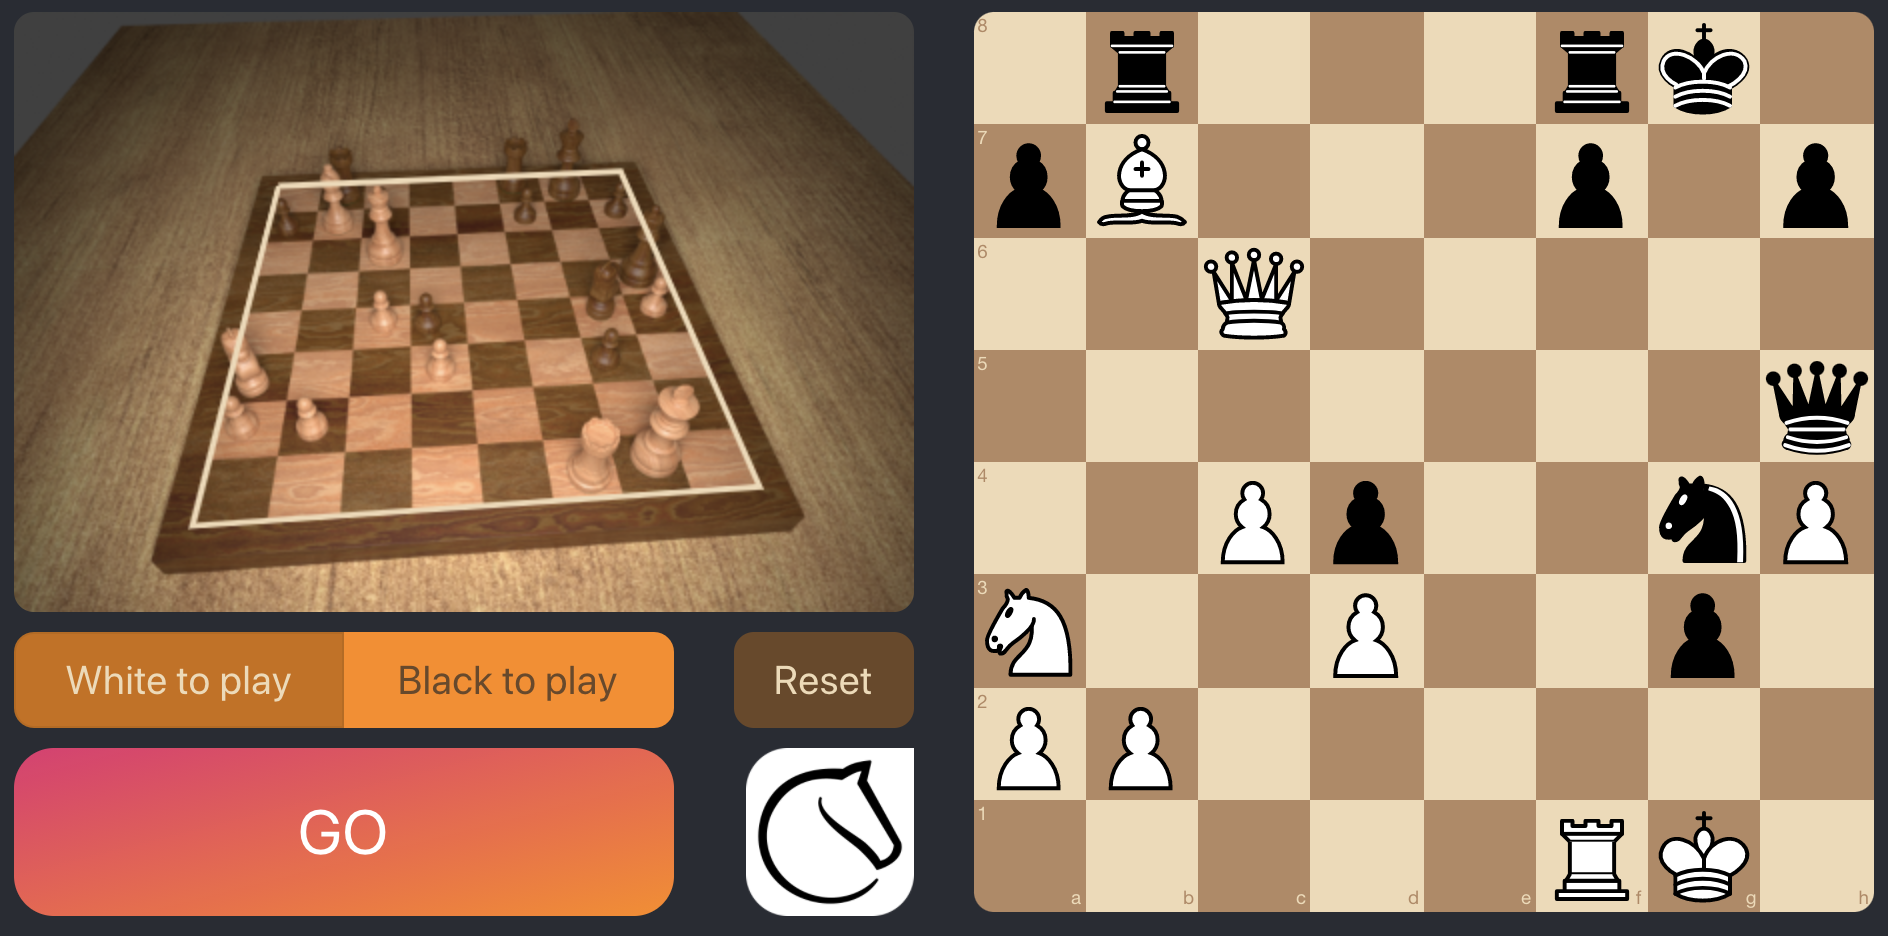
\includegraphics[width=\textwidth]{screenshot_chesscogapp_inference}
    \caption{Screenshot of the chess position inference using the web app.}
    \label{fig:chesscogapp_inference}
\end{figure}
The performance of the system was manually tested on a number of different chess positions from the test set in this fashion.
As per the second point, \cref{chap:chess_recognition,chap:adapting,chap:evaluation} carry out empirical performance evaluations and analyse the results.
Finally, the next section provides some more details about the automated testing procedure as per the last point.

\section{Automated testing}
All three repositories contain automated unit tests.
Instructions for executing these tests are provided in \cref{sec:recap_tests,sec:chesscog_tests,sec:chesscogapp_tests}.
As explained in \cref{chap:implementation}, they are run on every commit by a \gls{ci} pipeline.
\Cref{lst:tests_recap,lst:tests_chesscog,lst:tests_chesscogapp} show the command line output obtained when running each repository's test suite manually.
\begin{listing}
    \verbatiminput{data/tests/recap.txt}
    \caption{Automated tests for the \texttt{recap} package.}
    \label{lst:tests_recap}
\end{listing}%
\begin{listing}
    \verbatiminput{data/tests/chesscog.txt}
    \caption{Automated tests for the \texttt{chesscog} package.}
    \label{lst:tests_chesscog}
\end{listing}%
\begin{listing}
    \begin{sublisting}[b]{\textwidth}
        \verbatiminput{data/tests/chesscog-app.txt}
        \caption{tests for the backend \acs{api} (Python)}
    \end{sublisting}
    \medskip\par
    \begin{sublisting}[b]{\textwidth}
        \verbatiminput{data/tests/chesscog-app-node.txt}
        \caption{tests for the frontend \acs{gui} (Node)}
    \end{sublisting}
    \caption{Automated tests for the web app.}
    \label{lst:tests_chesscogapp}
\end{listing}%
These outputs show that the submitted versions of each of the packages pass all the tests.
The Python tests were written using the \texttt{pytest} framework and the frontend tests for the web app use \texttt{jest} for Node.
To test the frontend \gls{gui}, the \texttt{jest} tests mock up the backend \gls{api} with fake responses in order to test that the desired output is rendered to the \gls{dom}.

\end{document}